\documentclass[journal]{IEEEtran}

\usepackage{epsfig}
\usepackage{graphicx}
\usepackage{url}
\usepackage{cite}
\usepackage{epstopdf}
\usepackage{subcaption}
\usepackage{amsmath}
\usepackage{multirow}


\begin{document}


\title{I Think What I Hear, The Influence of Social Media on Political Ideologies}


\author{
	\IEEEauthorblockN{
		\textbf{Richard Matovu and Zakery Fyke \\ 
			Texas Tech University, Lubbock, TX, US}
	}
}

% The paper headers
\markboth{CS 5331 - Data Analytics Project by Dr. Fang Jin}%
{Shell \MakeLowercase{\textit{et al.}}: Bare Demo of IEEEtran.cls for IEEE Journals}


% make the title area
\maketitle



% For peer review papers, you can put extra information on the cover
% page as needed:
% \ifCLASSOPTIONpeerreview
% \begin{center} \bfseries EDICS Category: 3-BBND \end{center}
% \fi
%
% For peerreview papers, this IEEEtran command inserts a page break and
% creates the second title. It will be ignored for other modes.
\IEEEpeerreviewmaketitle



	\section{Introduction}

	The current political atmosphere across the world has changed. The results of the 2016 Presidential Election and the 2016 Brexit vote in the United Kingdom surprised many, defying prediction models and expectations of voters across both countries. Politics in the United States has become heavily divided between the two main parties, the Republicans and the Democrats, and some experts believe that the shock from the election results can be attributed to the formation of Echo Chambers in the public sphere, often blaming the widespread use of social media and other electronic communication methods for their existence.\cite{npr}\cite{cnn}\cite{nyt}.
	
	Echo Chambers are the metaphorical description given to the situation in which beliefs, information, and ideas are reinforced or cemented inside a defined system. A common example is an individual exclusively associating themselves with those who agree with or share their ideals and their point of view. The Echo Chamber reinforces one’s own present world view because of the lack of exchange of dialogue with those who hold a different point of view. The advent of Social Media has allowed Echo Chambers to be formed more easily than ever, and with over 60\% of Americans getting their news from Social Media according to a study by Pew Research Center \cite{pew}, this problem could be getting worse. Analysis of the data found on Twitter may allow us to locate these Echo Chambers present based on the political party divide.
	
	\section{Motivation}
	
	Social Echo Chambers have become a hot topic, especially in public media, as many believe that the formation of Echo Chambers is leading to a radicalization of political views on both sides of the party divide, making it more and more difficult for both sides to find a common ground, and leading to social unrest. This inability to find common ground between the two parties makes it more and more difficult for the two to find compromises that both sides will accept, leading to events like the 2013 Shutdown of the Federal Government when both sides were unable to find a compromise on the Federal Debt Ceiling. 
	
	This tendency of similar and like minded individuals to form ties with one another in a form of Confirmation Bias is also known as homophily. The phenomenon which causes this is often cited as cognitive dissonance and selective exposure theories, well researched and explained areas of human psychology. According to these theories, people experience positive feeling when they are presented with information which confirms their already held opinions on the subject. When faced with opinions which conflict with their own, humans are more likely to experience stress and a pressure to conform. This leads to individuals being more likely to seek out others who agree with them and to find information and discussions which reinforce their original and already held view. This leads to individuals grouping together into smaller homogeneous groups out of the overall public sphere, affiliating with other individuals with similar beliefs, educations, and world views. It follows, then, that the Echo Chamber effect is caused by this tendency of individuals desiring to create homogeneous groups, intentionally or otherwise, by exclusively affiliating with individuals whom share their own political view. 
	
	We are interested in seeing if we can find and visualize the formation of these Echo Chambers by utilizing the information available on social media, namely by analyzing tweets and followers found on Twitter. Twitter is one of the largest Social Media platforms in the world, and with the politically charged atmosphere currently present in the United States, we believe we will be able to find lots of data which will help us identify these Echo Chambers. Is it possible to visualize the formation of these Echo Chambers on Twitter by analyzing the data we gather? If so, can we find what factors lead to the formation of these Echo Chambers and possibly identify some common ground between the two parties that might be used to break them? 
	
	\section{Related Work}
	
	The effects of conversations happening in cyberspace have a very real and measurable impact in the real world. Hampton et al \cite{hampton} found in 2016 that “Twitter users who felt their audience on Twitter agreed with their opinion were more willing to speak out on that issue in the workplace”. There have been numerous methodologies used to locate and visualize the Echo Chambers that become present online and on social media, including analyzing blog posts and the comments on those posts and analyzing the messages and connections found on Twitter and Facebook. 

	The topic of whether or not ideological polarization is exhibited in online exchanges is still an open debate among researchers. Conover et al \cite{conover} found that political ideology could be predicted with a high level of accuracy by analyzing tweets of the users. By contrast, Bakshy et al \cite{Bakshy1130} found that there was very little online ideological segregation in absolute terms, with open exchanges and exposure to ideological differences being fairly common for nonpolitical issues. Variations like these are common between studies, and one reason for them might be that some studies use a self-selected sample of partisan individuals, while other studies have not. 
	
	With some similarity to the topic of whether ideological polarization even exists in online exchanges, which side of the political spectrum would be more likely to engage in selective exposure to information -- information which confirms the opinions which they already hold -- is still an open topic with a variety of answers from different researchers. While not the direct focus of our studies, it should be noted in the peripheral that different studies have found different results. The ones performed by Bakshy et al \cite{Bakshy1130} found that liberals are much more likely than conservatives to engage in cross-ideological dissemination of political and nonpolitical information, which stands in contrast to the rising belief of many that liberals, especially those on college campuses, have formed their own echo chambers. Colleoni et al \cite{colleoni} found that Democrats exhibit higher levels of political homophily, indicative of an Echo Chamber, but that Republicans that follow official Republican accounts exhibit higher levels still.
	
	In the past, previous work has analyzed the presence of Echo Chambers forming around online blogs. Gilbert et al \cite{gilbert} found in their study that blogs frequently created what they defined to be an Echo Chamber, with certain genres of blogs being more likely to meet these conditions. However, their metric for deciding if a blog could be categorized as an Echo Chamber was based on the ratio of comments left on posts which agreed with the writer of the blog. As they mention, there is no agreed upon metric which designates something as an Echo Chamber. 

	Adamic and Glance \cite{adamic} analyzed the differences in behavior of liberal and conservative blogs and how frequently one referred to another. They chose 1000 political blogs, and analyzed the top 20 conservative and top 20 liberal blogs, ranking them based on the number of citations each blog received from October and November of 2004, the period of the George W. Bush vs John Kerry Presidential election. From these 40 blogs, they collected roughly 23,000 posts from 8/29/04 - 11/15/04, with a slight bias in the count towards the left leaning blogs. During analysis, they found that conservative blogs link to one another more frequently than liberal blogs, but that particular liberal blogs are more likely to be linked to by other left leaning blogs. Their analysis also showed that only 15 percent of all links were bipartisan. 
	
	More recent work has begun to focus on the influence of Social Media on the public sphere and on the formation of Echo Chambers. Twitter has been the focus of most of these studies, due to the ease of access for information on users and their corresponding tweets. The content of tweets often proves to be easier to analyze as well; because they are limited to 140 characters, tweets must be short and to the point, allowing for easier topic modeling. 
	
	Barberá et al \cite{barbera} analyzed a collection of 3.8 million Twitter users in the United States. They pointed out that methods which focus on analyzing the content of Twitter messages in order to draw conclusions was not scalable, bringing up questions about the validity of any conclusions made by these techniques. Instead, they focused on Latent Space Modeling, focusing on the connections between different Twitter users and their retweeting, or sharing of tweets, in order to draw their conclusions. They also chose 12 significant, political and nonpolitical, events from the period of 2012 to 2014, including the United States Federal Budget, Marriage Equality, the Winter Olympics, and the Academy Awards, and used these in order to collect roughly 150 million tweets which mentioned any of these keywords. 

	Using this collection of tweets, they found their 3.8 million active Twitter followers to analyze. By using known political pages, such as The Tea Party, Stephen Colbert, and others, they created a Latent Space Model of all these Twitter users.  Barberá et al \cite{barbera} concluded that while the Social Media sphere is not necessarily bounded by ideological contours, especially when it comes to nonpolitical issues like the Winter Olympics, when it comes to politicized issues, individuals are significantly more likely to pass on information to other users that they have received from sources which are similar to their existing network. 
	
	Williams et al \cite{williams} utilized a similar form of Network Analysis, collecting nearly 600,000 distinct tweets from nearly 180,000 distinct users regarding Climate Change by utilizing hashtags such as \textit{\#globalwarming, \#climatechange,} and \textit{\#climaterealists} to name a few in order to perform an analysis of social media debates regarding Climate Change. They created three separate social networks: "Follower" networks, "Retweet" networks, and "Mention" networks, where each was created from users following one another, retweeting each other's tweets, or mentioning one another in a tweet respectively. The most active users analyzed were classified by researchers as either activists, skeptics, neutral, or unknown. If researchers could not reach a unanimous decision, the user was marked as ambiguous. 

	They found in their study that there was a high degree of polarization in attitudes regarding climate change discussion on Twitter; users who were active in online discussions tended to have strong attitudes and users on Twitter were likely to self-segregate into like minded communities regarding the issue. This self segregation may be indicative of divides along overall political ideologies, instead of just the topic of Climate Change, but this study did not expand beyond just the single topic. 
	
	Colleoni et al \cite{colleoni} utilized data collected by Kwak et al \cite{kwak} in 2009 which consists of all nodes and ties on Twitter in 2009, where nodes are individual users and ties represent the relationships between them. This dataset consists of over 40 million nodes and 1.47 billion ties, though because it is almost a decade out of date, this number has certainly grown considerably since then. They also utilized a collection of 467 million tweets from a 7 month period from June 1st to December 31st, 2009 collected by Yang and Leskovec \cite{yang}, utilizing training data containing 60,000 political and 170,000 nonpolitical titles from news blogs. They also utilized a training set containing 1,683 Democrat users and 8,868 Republican users, assuming that users who are following exclusively Republicans or Democrats are themselves Republicans or Democrats. 

	They used this collection of data in order to predict the political orientation of users from the content they shared, with an accuracy of roughly 0.96 for Republicans and 0.79 for Democrats, identifying 72,302 Republicans, and 782,371 Democrats. Using this, they measured the political homophily by defining it as the number of outbound ties (that is, directed to users with similar political orientation plus directed to users with different political orientation). While they concluded that Democrats in general had higher levels of homophily than Republicans, except when considering Republicans which follow official Republican sources, they also had a heavily unbalanced dataset overall, with far more Democrats than Republicans identified, despite having far more Republicans than Democrats in their training data. 
	
	\section{Methodology}
	
	To complete this task, we have collected data from Twitter through web crawling techniques including, but not limited to, the Twitter API for R and Python. This data has been gathered from the top ten United States Senators which have the largest following on Twitter, measured by number of followers according to \cite{senatorFollowers}, as their political affiliation is already established, as are their Twitter handles. From these accounts, we collected data regarding their tweets and their Twitter followers. We then analyzed this data we collected by comparing the collections of each politician's followers to see if those who follow a particular influential member of Congress from one party are less likely to follow members of the other party. 
	
	
	%Idk what we wanna do with this paragraph since we aren't doing this at all. 
	%Expanding upon this, we will then attempt to visualize who the followers of these politicians are following, so that we can get a total view of any sort of Echo Chamber that may have been formed between these groups. For example, might we find that those Twitter users who follow a particular party are very unlikely to follow particular celebrities or corporate leaders? With this, we can classify the followers of these politicians into different Echo Chambers. 
	
	%Once this visualization has been done, we will then attempt to identify which topics are important to each of our groups and the sentiment which they have towards this topic. For example, both sides may frequently discuss issues like Gun Control, but one group may have a negative outlook on it, while the other may have a positive outlook on it. We will then use this analysis to attempt to predict which of our Echo Chambers a person falls into based on their tweets contained in our dataset from the Presidential Campaign.
	
	\subsection{Dataset}
	
	For our dataset, we have collected a subset of 500,000 followers from each of our ten US Senators twitter accounts, for a total of 3,338,398 unique users shared across all accounts, with Republican Senators having 1,678,040 unique followers, and Democrat Senators having 2,167,455 unique followers. Individual follower counts for each senator are given in Table \ref{senatorTable}.
	
	For each of the ten senators, we also harvested up to 3,200 tweets via the Twitter API, starting with their most recent tweets. This came up to 12,663 tweets from Republican Senators, and 18,622 tweets for Democrat Senators, for a total of 31,255 tweets overall.
	
	\begin{table}[htp]
		\centering
		\caption{Followers by Senator}
		\label{senatorTable}
		\begin{tabular}{ll|lll}
			\hline
			Republicans & Followers & Democrats        & Followers &  \\ \hline
			Marco Rubio (FL) & 3,123,752 & Bernie Sanders(VT)   & 6,398,668 &  \\
			John McCain (AZ) & 2,626,424 & Elizabeth Warren (MA) & 3,203,264 &  \\
			Rand Paul (KY)   & 1,503,933 & Cory Booker (NJ)      & 3,442,808 &  \\
			Ted Cruz  (TX)  & 1,022,515 & Chuck Schumer (NY)   & 937,391   &  \\
			&           & Kamala Harris (CA)    & 836,202   &  \\
			&           & Tim Kaine (VA)        & 693,484   &  \\ \cline{1-5}
		\end{tabular}
	\end{table}
	
	\subsection{Implementation}
	
	First, we analyzed the list of Twitter followers of the ten most influential US Senators on Twitter, measured by their number of followers. These senators included Elizabeth Warren, Bernie Sanders, and Ted Cruz, among others. We then compared these list of followers to find if followers of one political party are less likely to follow the members of the other. This was indeed the case and, in addition, we found that, in general, Democrats were less likely than Republicans to follow senators of the other party, but that Republicans who followed all top members of their party were less likely than Democrats to follow senators from the other party. We then visualized this information utilizing Python.  
	
	Once this was completed, we then analyzed the Tweets sent out by these ten United States Senators to find the topics which each discussed most frequently, finding that, as expected, both parties discussed different topics on Twitter. This topic analysis was performed by utilizing Latent Dirichlet Allocation, which is detailed in the paper by Blei et al \cite{blei}. 
	
	Forming a training and testing set from our original Echo Chamber model, based on who is following who, we can then use our analysis of the topics each side finds important to classify tweets based on their messages, without having to have knowledge of who the person is following. 
	
	\section{Discussion}	

	We analyzed the number of followers who followed exclusively Republicans and Democrats. Out of 1,678,040 followers who followed at least one of our four Republicans, we found that 1,220,940, almost 73 percent, do not follow any of our six Democrats. Similiarly, we found that out of our 2,167,455 followers who followed at least one of our Democrats, 1,710,358, almost 79 percent, do not follow any of our four Republicans. We then narrowed this further, by examining those who are following all of the top members of a particular party. Out of 1,678,040 followers who followed at least one of our Republicans, we found that 11,393 followed all four of our Republican Senators. Of this 11,393, we found that 10,928, almost 96 percent, did not follow any of our Democrat Senators, meaning they exclusively followed the four Republicans. Similarly, of our 2,167,455 followers who followed at least one of our Democrats, we found that 6,498 followed all six of our Democrat Senators, and that 6,033, almost 93 percent, of these did not follow any of our Republican senators as shown in Figure \ref{fig:PartyFollowers}.

\begin{figure}[htp]
  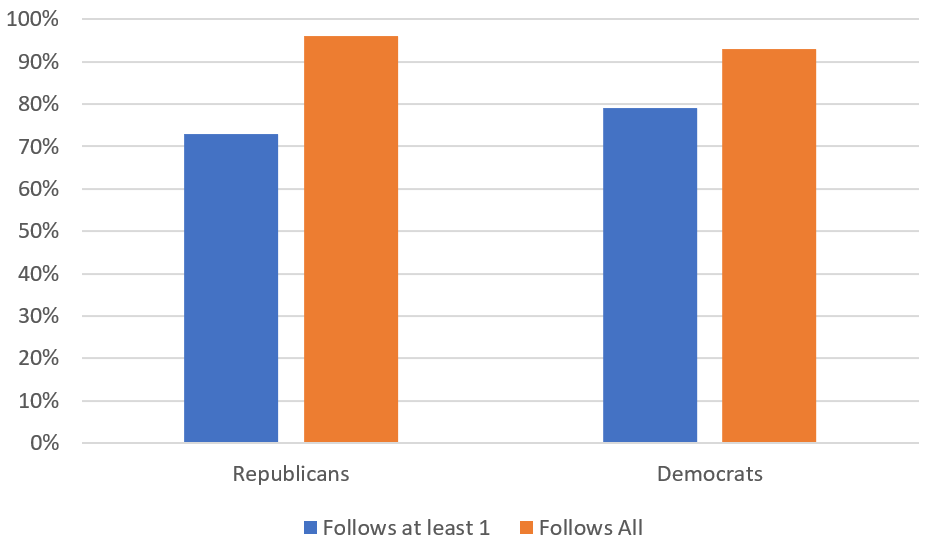
\includegraphics[width=0.9\linewidth]{partyFollowers.png}
  \caption{Distribution of party followers who exclusively follow a particular party.}
  \label{fig:PartyFollowers}
\end{figure}

	Figure \ref{fig:PartyFollowers} shows the party followers who follow a particular party's senators, but do not follow any of the other party's senators. The percentage of Twitter users who follow at least one Republican Senator and no Democrat Senators is lower than the percentage of users who follow at least one Democrat Senator and no Republican Senators. This potentially indicates that followers of Republican Senators are more likely to also follow Democrat Senators than followers of Democrat Senators are to follow Republican Senators. However, users who follow all four of our Republican Senators are less likely to follow any Democrat Senators than followers of all four of our Democrat Senators 

	\section{Conclusion}
	
	It seems that with each passing year, American politics and politics around the globe are becoming more and more divided along party lines, and each year it is becoming harder for the two sides to find compromises between them that will both parties happy, leading to more and more political strife as time goes by. The formation of Echo Chambers, which reinforce one's own worldview and make it more difficult to consider the validity of another person's view, have largely contributed to this. By utilizing the data collected from Twiter, we can identify the boundaries that exist along party lines, allowing us to identify these Echo Chambers and work together to find ways to break them. 


%\bibliographystyle{IEEEtran}
%\bibliography{IEEEabrv,references}

\end{document}
